\documentclass[preprint,a4paper,fleqn]{cas-dc}
\usepackage[authoryear,longnamesfirst]{natbib}
\usepackage{booktabs}
\usepackage{multirow}
\usepackage{amsmath}
\usepackage{siunitx}
\usepackage{graphicx}
\usepackage{hyperref}
\makeatletter
\def\fps@figure{t}
\makeatother

\begin{document}
\let\WriteBookmarks\relax
\def\floatpagepagefraction{1}
\def\textpagefraction{.001}

\shorttitle{Multi-layer Legal NLP for Criminal Labor-Law Decisions}
\shortauthors{Author et al.}

\title[mode=title]{A Multi-Layer Framework for Filtering, Merit Classification, Sentence Segmentation, and Named-Entity Extraction in Brazilian Criminal Labor-Law Decisions}

\author[1]{Carlos A. V. Tinin}
\cormark[1]
\ead{carlostinin@gmail.com}
\credit{Conceptualization, Methodology, Software, Writing -- original draft}

\author[1,2]{Edison P. de Freitas}
\ead{edison.pignaton@inf.ufrgs.br}
\credit{Validation, Formal analysis, Writing -- review \& editing}

\author[3]{Kevin H. M. Gularte}
\ead{kevinhmg@gmail.com}
\credit{Validation, Formal analysis, Writing -- review \& editing}

\author[4]{Elena J. da Costa}
\ead{elena.javidi@ufrgs.br}
\credit{Validation, Formal analysis, Writing -- review \& editing}

\author[4]{João Paulo J. da Costa}
\ead{joao.costa@ufrgs.br}
\credit{Validation, Formal analysis, Writing -- review \& editing}

\affiliation[1]{organization={Federal University of Rio Grande do Sul (UFRGS)},
            city={Porto Alegre},
            postalcode={90010-150},
            state={RS},
            country={Brazil}}

\affiliation[2]{organization={Halmstad University},
            city={Halmstad},
            postalcode={30118},
            state={Halland},
            country={Sweden}}

\affiliation[3]{organization={University of Brasília (UnB)},
            city={Brasília},
            postalcode={70910-900},
            state={DF},
            country={Brazil}}

\affiliation[4]{organization={Hamm-Lippstadt University of Applied Sciences (HSHL)},
            city={Lippstadt},
            postalcode={59557},
            state={NRW},
            country={Germany}}

\cortext[1]{Corresponding author}

\begin{abstract}
This paper presents a multi-layer legal NLP framework for extracting structured information from Brazilian criminal labor-law judicial decisions related to modern slavery. Starting from a heterogeneous corpus (2,581 documents), the framework applies: (i) document-type filtering to retain only final decisions, (ii) legal-text normalization with task-specific outputs for classification and NER, (iii) penal-merit classification using Legal-BERT embeddings with classical classifiers, (iv) LLM-assisted sentence segmentation for conviction-focused documents, and (v) legal-domain NER for entity extraction. We describe the full pipeline, evaluation protocol, and error analysis, and discuss practical deployment constraints, reproducibility, and ethical/legal considerations. Results indicate that layered filtering and task-oriented preprocessing substantially improve downstream extraction quality in low-resource legal settings.
\end{abstract}

\begin{highlights}
\item Multi-layer filtering for noisy, heterogeneous legal corpora.
\item Task-specific normalization improves classification and NER compatibility.
\item Conviction-focused segmentation and legal-domain NER for structured extraction.
\item Reproducible benchmark design for Portuguese criminal labor-law decisions.
\end{highlights}

\begin{keywords}
Legal NLP \sep Information extraction \sep Named entity recognition \sep Judicial decisions \sep Modern slavery \sep Portuguese language resources
\end{keywords}

\maketitle

\section{Introduction}
\label{sec:introduction}
\subsection{Problem context and motivation}
\begin{itemize}
    \item Explain the supply-chain transparency challenge in modern slavery investigations.
    \item Justify why judicial decisions are high-value evidence sources.
\end{itemize}
\subsection{Research gap}
\begin{itemize}
    \item Existing legal NLP pipelines are often single-stage and not robust to document heterogeneity.
    \item Limited resources for Portuguese criminal labor-law datasets and benchmarks.
\end{itemize}
\subsection{Research questions}
\begin{itemize}
    \item RQ1: How much does multi-layer filtering improve downstream extraction reliability?
    \item RQ2: Which merit-classification model is most robust under class imbalance?
    \item RQ3: How do segmentation quality and NER quality interact in the final extraction output?
\end{itemize}
\subsection{Main contributions}
\begin{enumerate}
    \item End-to-end framework from raw legal documents to structured entities.
    \item Task-adaptive preprocessing design with separate outputs for classification and NER.
    \item Comparative evaluation of embedding-based classifiers for penal-merit prediction.
    \item Practical protocol for LLM-assisted segmentation plus legal-domain NER.
\end{enumerate}

\section{Related Work}
\label{sec:related}
\subsection{Legal document filtering and classification}
\subsection{Legal sentence segmentation and structure mining}
\subsection{Legal NER in low-resource languages}
\subsection{Comparative synthesis with at least three high-impact studies}
\textbf{Required output in this section:} a compact comparison table with dataset size, language, task formulation, model family, metrics, and limitations.

\section{Dataset and Problem Definition}
\label{sec:data}
\subsection{Corpus description}
\begin{itemize}
    \item Raw corpus size: 2,581 documents.
    \item Document heterogeneity (senten\c{c}a, ac\'ord\~ao, despacho, ata, etc.).
\end{itemize}
\subsection{Task definitions}
\begin{itemize}
    \item T1: Document-type filtering.
    \item T2: Penal-merit classification (classes: condena\c{c}\~ao, absolvi\c{c}\~ao, extinto).
    \item T3: Decision segmentation.
    \item T4: Named-entity extraction.
\end{itemize}
\subsection{Annotation and label governance}
\begin{itemize}
    \item Define legal criteria for label assignment (Art. 149 framing).
    \item Report annotation process and expert validation protocol.
\end{itemize}
\subsection{Data governance and ethics}
\begin{itemize}
    \item LGPD/privacy handling, anonymization strategy, and legal-compliance statement.
\end{itemize}

\section{Methodology}
\label{sec:methodology}
\subsection{Overview of the multi-layer pipeline}
Figure~\ref{fig:activity_pipeline} presents the end-to-end workflow adopted in this study. The process starts with document-type normalization and filtering (Stage1\_1), keeping only judicial sentences that are relevant to criminal-merit analysis. Next, Stage1\_2 applies task-adaptive preprocessing and generates two normalized outputs: one optimized for merit classification and one that preserves legal-text patterns for segmentation and NER. Stage2 performs penal-merit classification, Stage3 applies LLM-assisted segmentation to the conviction subset, and Stage4 performs legal-domain named-entity extraction over segmented content.

\begin{figure*}
    \centering
    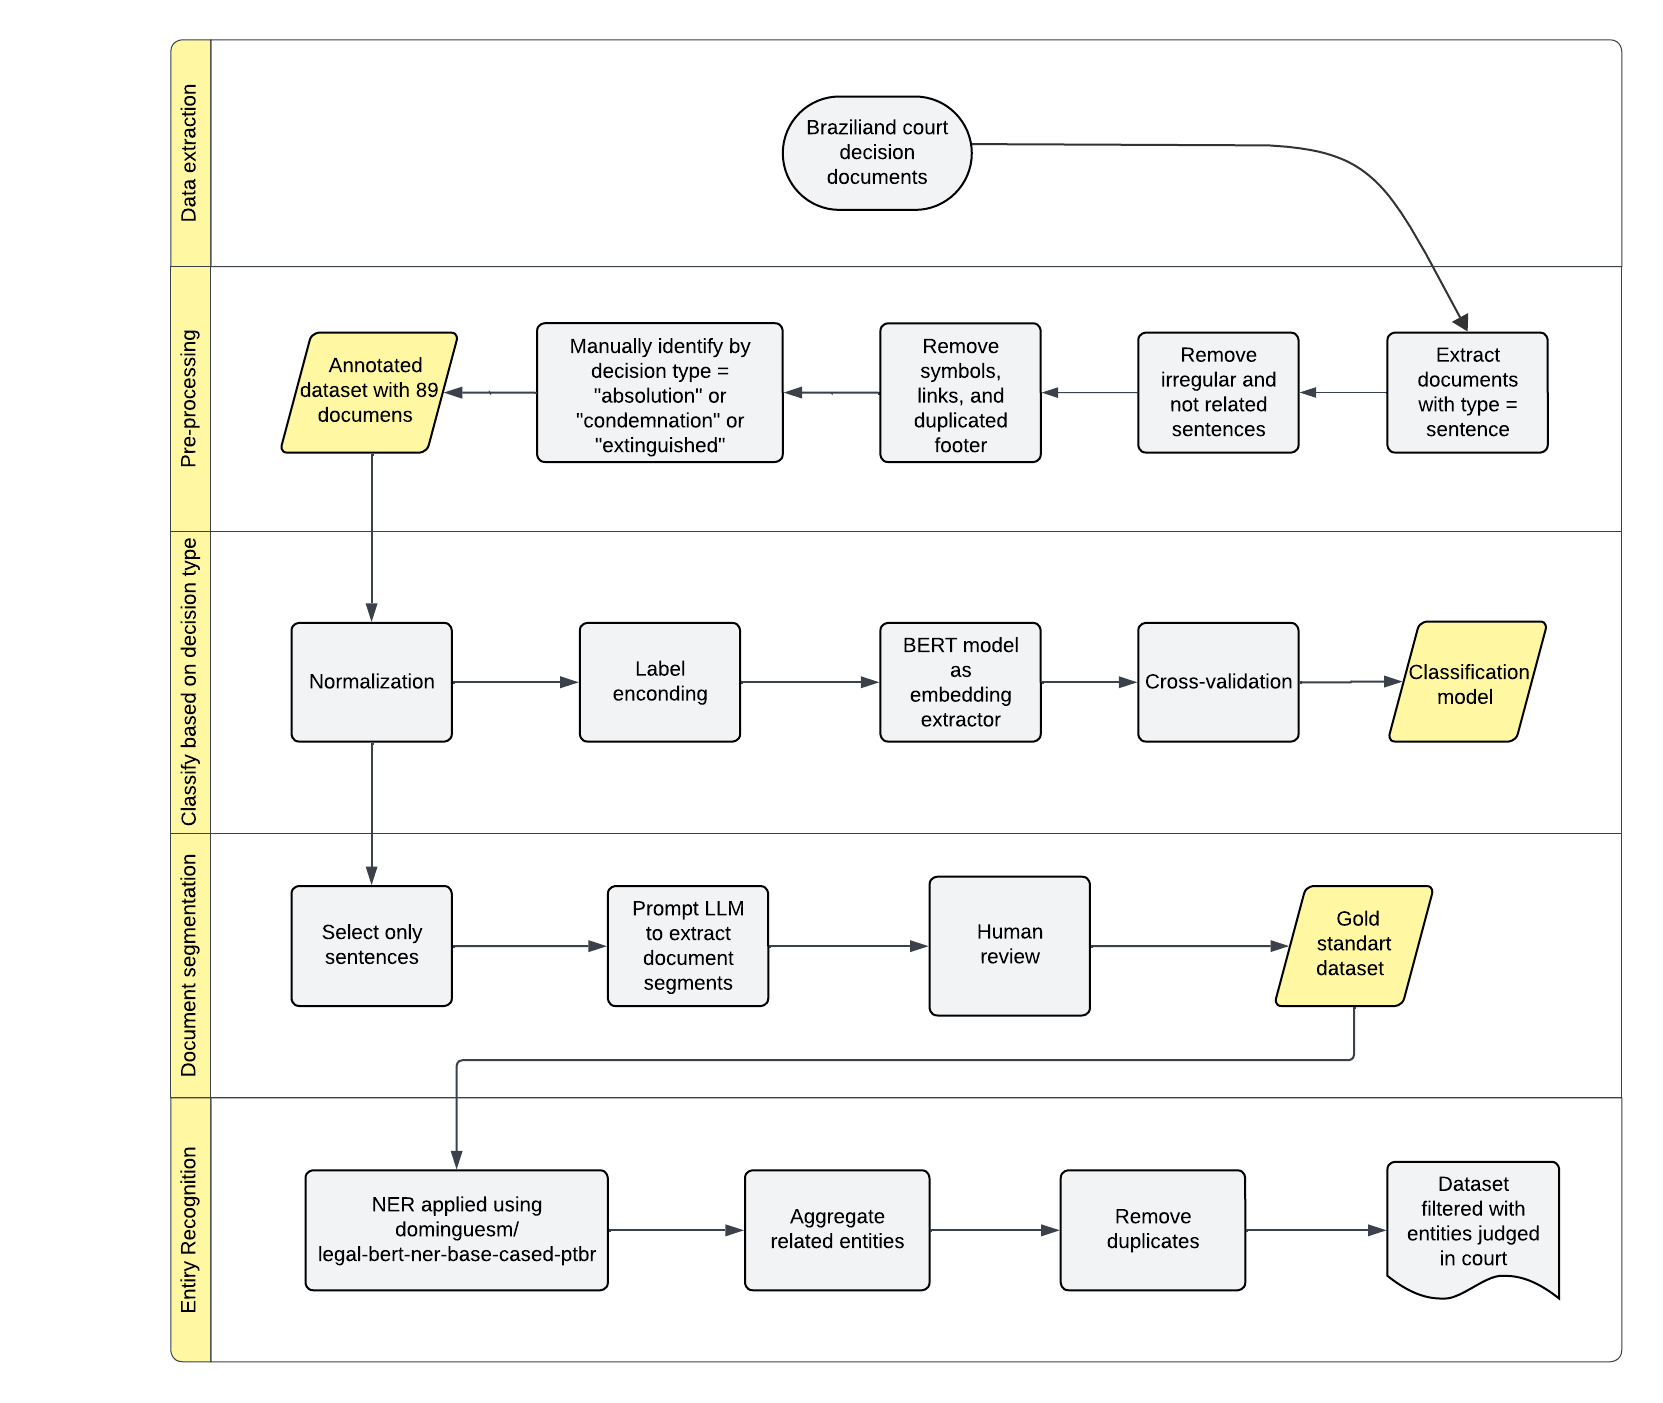
\includegraphics[width=0.98\linewidth]{figs/activity_diagram.png}
    \caption{Activity diagram of the proposed multi-layer pipeline for legal document filtering, penal-merit classification, segmentation, and NER extraction.}
    \label{fig:activity_pipeline}
\end{figure*}

\subsection{Stage1\_1: Document-type normalization and filtering}
\begin{itemize}
    \item Pattern-based extraction of document type from metadata-like spans.
    \item Final retention of \textit{senten\c{c}a} documents.
\end{itemize}

\subsection{Stage1\_2: Task-adaptive legal text preprocessing}
\begin{itemize}
    \item PJe duplicate-footer removal.
    \item Aggressive normalization for classification output.
    \item Conservative normalization for NER/segmentation output.
\end{itemize}

\subsection{Stage2: Penal-merit classification with Legal-BERT embeddings}
\begin{itemize}
    \item Encoders avaliados: \texttt{dominguesm/legal-bert-base-cased-ptbr}, \texttt{neuralmind/bert-base-portuguese-cased} e \texttt{neuralmind/bert-large-portuguese-cased}.
    \item Classifiers: Logistic Regression, linear SVM, Random Forest, XGBoost.
    \item Stratified $k$-fold protocol and weighted metrics.
\end{itemize}

\subsection{Stage3: LLM-assisted segmentation of conviction decisions}
\begin{itemize}
    \item Input restricted to conviction subset.
    \item Prompting protocol and JSON schema validation.
    \item Retry/failure handling and quality-control checks.
\end{itemize}

\subsection{Stage4: Legal-domain NER extraction}
\begin{itemize}
    \item Model: \texttt{dominguesm/legal-bert-ner-base-cased-ptbr}.
    \item Entity aggregation strategy and output schema.
\end{itemize}

\section{Experimental Setup}
\label{sec:experiments}
\subsection{Evaluation protocol}
\begin{itemize}
    \item Data splits, fold strategy, seeds, and confidence intervals.
    \item Primary metrics: macro-F1, weighted-F1, precision, recall, per-class scores.
\end{itemize}

\subsection{Baselines and ablations}
\begin{itemize}
    \item Baseline without multi-layer filtering.
    \item Baseline with single normalization stream.
    \item Ablation removing each stage (one-at-a-time).
\end{itemize}

\subsection{Implementation details}
\begin{itemize}
    \item Software stack, hardware profile, runtime, and cost profile (LLM calls).
\end{itemize}

\section{Results}
\label{sec:results}
\subsection{Merit classification performance}
Table~\ref{tab:encoder_comparison} compares three encoder backbones under the same downstream classifiers, using weighted F1 as the primary criterion. The best overall result is highlighted in bold and corresponds to BERTimbau-large with linear SVM ($F1=0.6152 \pm 0.0808$). Legal-BERT remains competitive and obtains the strongest XGBoost result ($F1=0.6114 \pm 0.0871$), while BERTimbau-base shows gains for Logistic Regression and Random Forest.

In practical terms, this indicates that domain adaptation in the encoder remains beneficial for the XGBoost configuration, while larger general-purpose Portuguese encoders can provide stronger performance with linear classifiers. Given this trade-off, both Legal-BERT+XGBoost and BERTimbau-large+SVM should be considered viable Stage2 operating points depending on interpretability and computational constraints.

\begin{table*}[t]
\centering
\caption{Stage2 encoder comparison across downstream classifiers (weighted F1, mean $\pm$ std across folds).}
\label{tab:encoder_comparison}
\begin{tabular}{lccc}
\toprule
Classifier & Legal-BERT (dominguesm) & BERTimbau-base (neuralmind) & BERTimbau-large (neuralmind) \\
\midrule
XGBoost & $0.6114 \pm 0.0871$ & $0.5261 \pm 0.0590$ & $0.5661 \pm 0.0558$ \\
SVM (Linear) & $0.5415 \pm 0.0484$ & $0.5350 \pm 0.0664$ & $\mathbf{0.6152 \pm 0.0808}$ \\
Random Forest & $0.5406 \pm 0.1249$ & $0.5611 \pm 0.0622$ & $0.5284 \pm 0.0420$ \\
Logistic Regression & $0.5399 \pm 0.0522$ & $0.5627 \pm 0.0613$ & $0.6136 \pm 0.0799$ \\
\bottomrule
\end{tabular}
\end{table*}

TODO: Mention that the BERT models were not fine-tuned for this specific case due to the limited amount of available data.

\subsection{Segmentation quality}
Report schema-valid rate, section-level agreement, and representative errors.

\subsection{NER extraction quality}
Report entity-level precision/recall/F1 (strict and relaxed matching if possible).

\subsection{End-to-end pipeline gains}
Compare extraction quality before vs. after multi-layer filtering.

\section{Discussion}
\label{sec:discussion}
\subsection{Why the pipeline works}
\subsection{Failure modes and error taxonomy}
\subsection{Generalization to other legal domains/languages}
\subsection{Operational and policy implications}

\section{Threats to Validity}
\label{sec:validity}
\begin{itemize}
    \item Internal validity: label noise, annotation drift, prompt sensitivity.
    \item External validity: transfer to other courts, years, and jurisdictions.
    \item Construct validity: legal meaning vs. NLP proxy metrics.
\end{itemize}

\section{Reproducibility Statement}
\label{sec:reproducibility}
\begin{itemize}
    \item Public code structure, dependency pinning, random seeds, and artifact inventory.
    \item Which resources can/cannot be publicly shared due to legal constraints.
\end{itemize}

\section{Conclusion and Future Work}
\label{sec:conclusion}
\begin{itemize}
    \item Summarize empirical and practical contributions.
    \item Future work: active learning, expert-in-the-loop verification, and cross-court transfer evaluation.
\end{itemize}

\section*{Acknowledgments}
Funding and institutional acknowledgments.

\printcredits
\bibliographystyle{cas-model2-names}
\bibliography{cas-refs}

\end{document}
